\documentclass[12pt,letterpaper]{article}
\usepackage{anysize}
\usepackage{amsmath}
\marginsize{2cm}{2cm}{1cm}{1cm}
\usepackage{listings}
\usepackage{cite}
\usepackage{caption}
\usepackage{upquote}
\usepackage{xcolor}
\usepackage{xcolor}

\usepackage{tikz}
\def\checkmark{\tikz\fill[scale=0.4](0,.35) -- (.25,0) -- (1,.7) -- (.25,.15) -- cycle;} 

\usepackage{graphicx}


\begin{document}

\begin{titlepage}
    \vspace*{4cm}
    \begin{flushleft}
    {\huge
        CS519 Shaders Final Project\\[.5cm]
    }
    {\large
        A simple Water simulation\\
	}
    \end{flushleft}
    \vfill
    \rule{5in}{.5mm}\\
    Li Li

\end{titlepage}
\section{source files}
There are:
\begin{tabular}{ |l | c |}
  \hline                       
  \textbf{Source file} & \textbf{what are they doing} \\ \hline
  mainwindow.cpp and mainwindow.h & activate the program from user\\ \hline
  glwidget.cpp and glwidget.h& handle creating windows in a certain OS \\ \hline
  camera.cpp and camera.h & do stuff to manipulate the camera  \\ \hline
  waterengine.cpp and waterengine.h & where truly  the water creating and rendering happened \\ \hline
  vector.h & telling how to do vector operation \\ \hline
\end{tabular}

\section{main steps}

\begin{itemize}
\item \textbf{Reading} My program is based on \textit{GPU Gems: Chapter 1. Effective Water Simulation from Physical Models.} Most of it is talking at water simulation. 
\item \textbf{Single Wave Function} As shown in figure1. We calculate Wavelength (L) ,Amplitude (A), Speed (S) and Direction (D ). In my implementation, D is random, A is set as 0.03f. L is from 0.3 to 0.8. Speed calculate as $S = 0.05 \times \sqrt[2]{\pi/L}$. And last part steepness is $ Steepness = 5.0\times (\textit{random-a-float}\times 2.0+1.0)$.

\item \textbf{Unit Normal Map} This is what I want to calculate in first pass program, an than apply them to second pass-program to the geometry to do a local bump mapping. See figure2 for whole flow chart.
\item \textbf{In Waterunit frag shader}, base on the equation (figure3).I calculated A, $\omega$ ,$\phi$ , D ,k to get the Normal of a certain point. Then it emits this normals to a normal map. Each one is compute comes from 50 waves.
\item \textbf{Compute Gerstner Waves vertex in waterrender vertex shader}, these are similar but only comes from 6 waves. See figure4,5,6 for the equation. Than it output the final geometry light vector to a vertex, and eye vertex to the vertex, as well as its texture parameter to following fragment shader.
\item \textbf{Final decision to the color of water: mixing specular and fresnel effect} The shader grab N from normal map that pass in as texture. And than obtain specular vector. For fresnel, it blend oceanbue and skyblue, and it is base on the view vector to it.$fresnel = R_{0} + (1.0 - R_{0}) * {1.0 - {-normalize(viewv)}\cdot {N}}^{5.0}$


\end{itemize}
\begin{figure}[p]
    \centering
    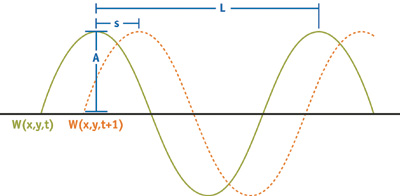
\includegraphics[width=1.0\textwidth]{fig1.jpg}
    \caption{A single wave}
\end{figure}
\begin{figure}[p]
    \centering
    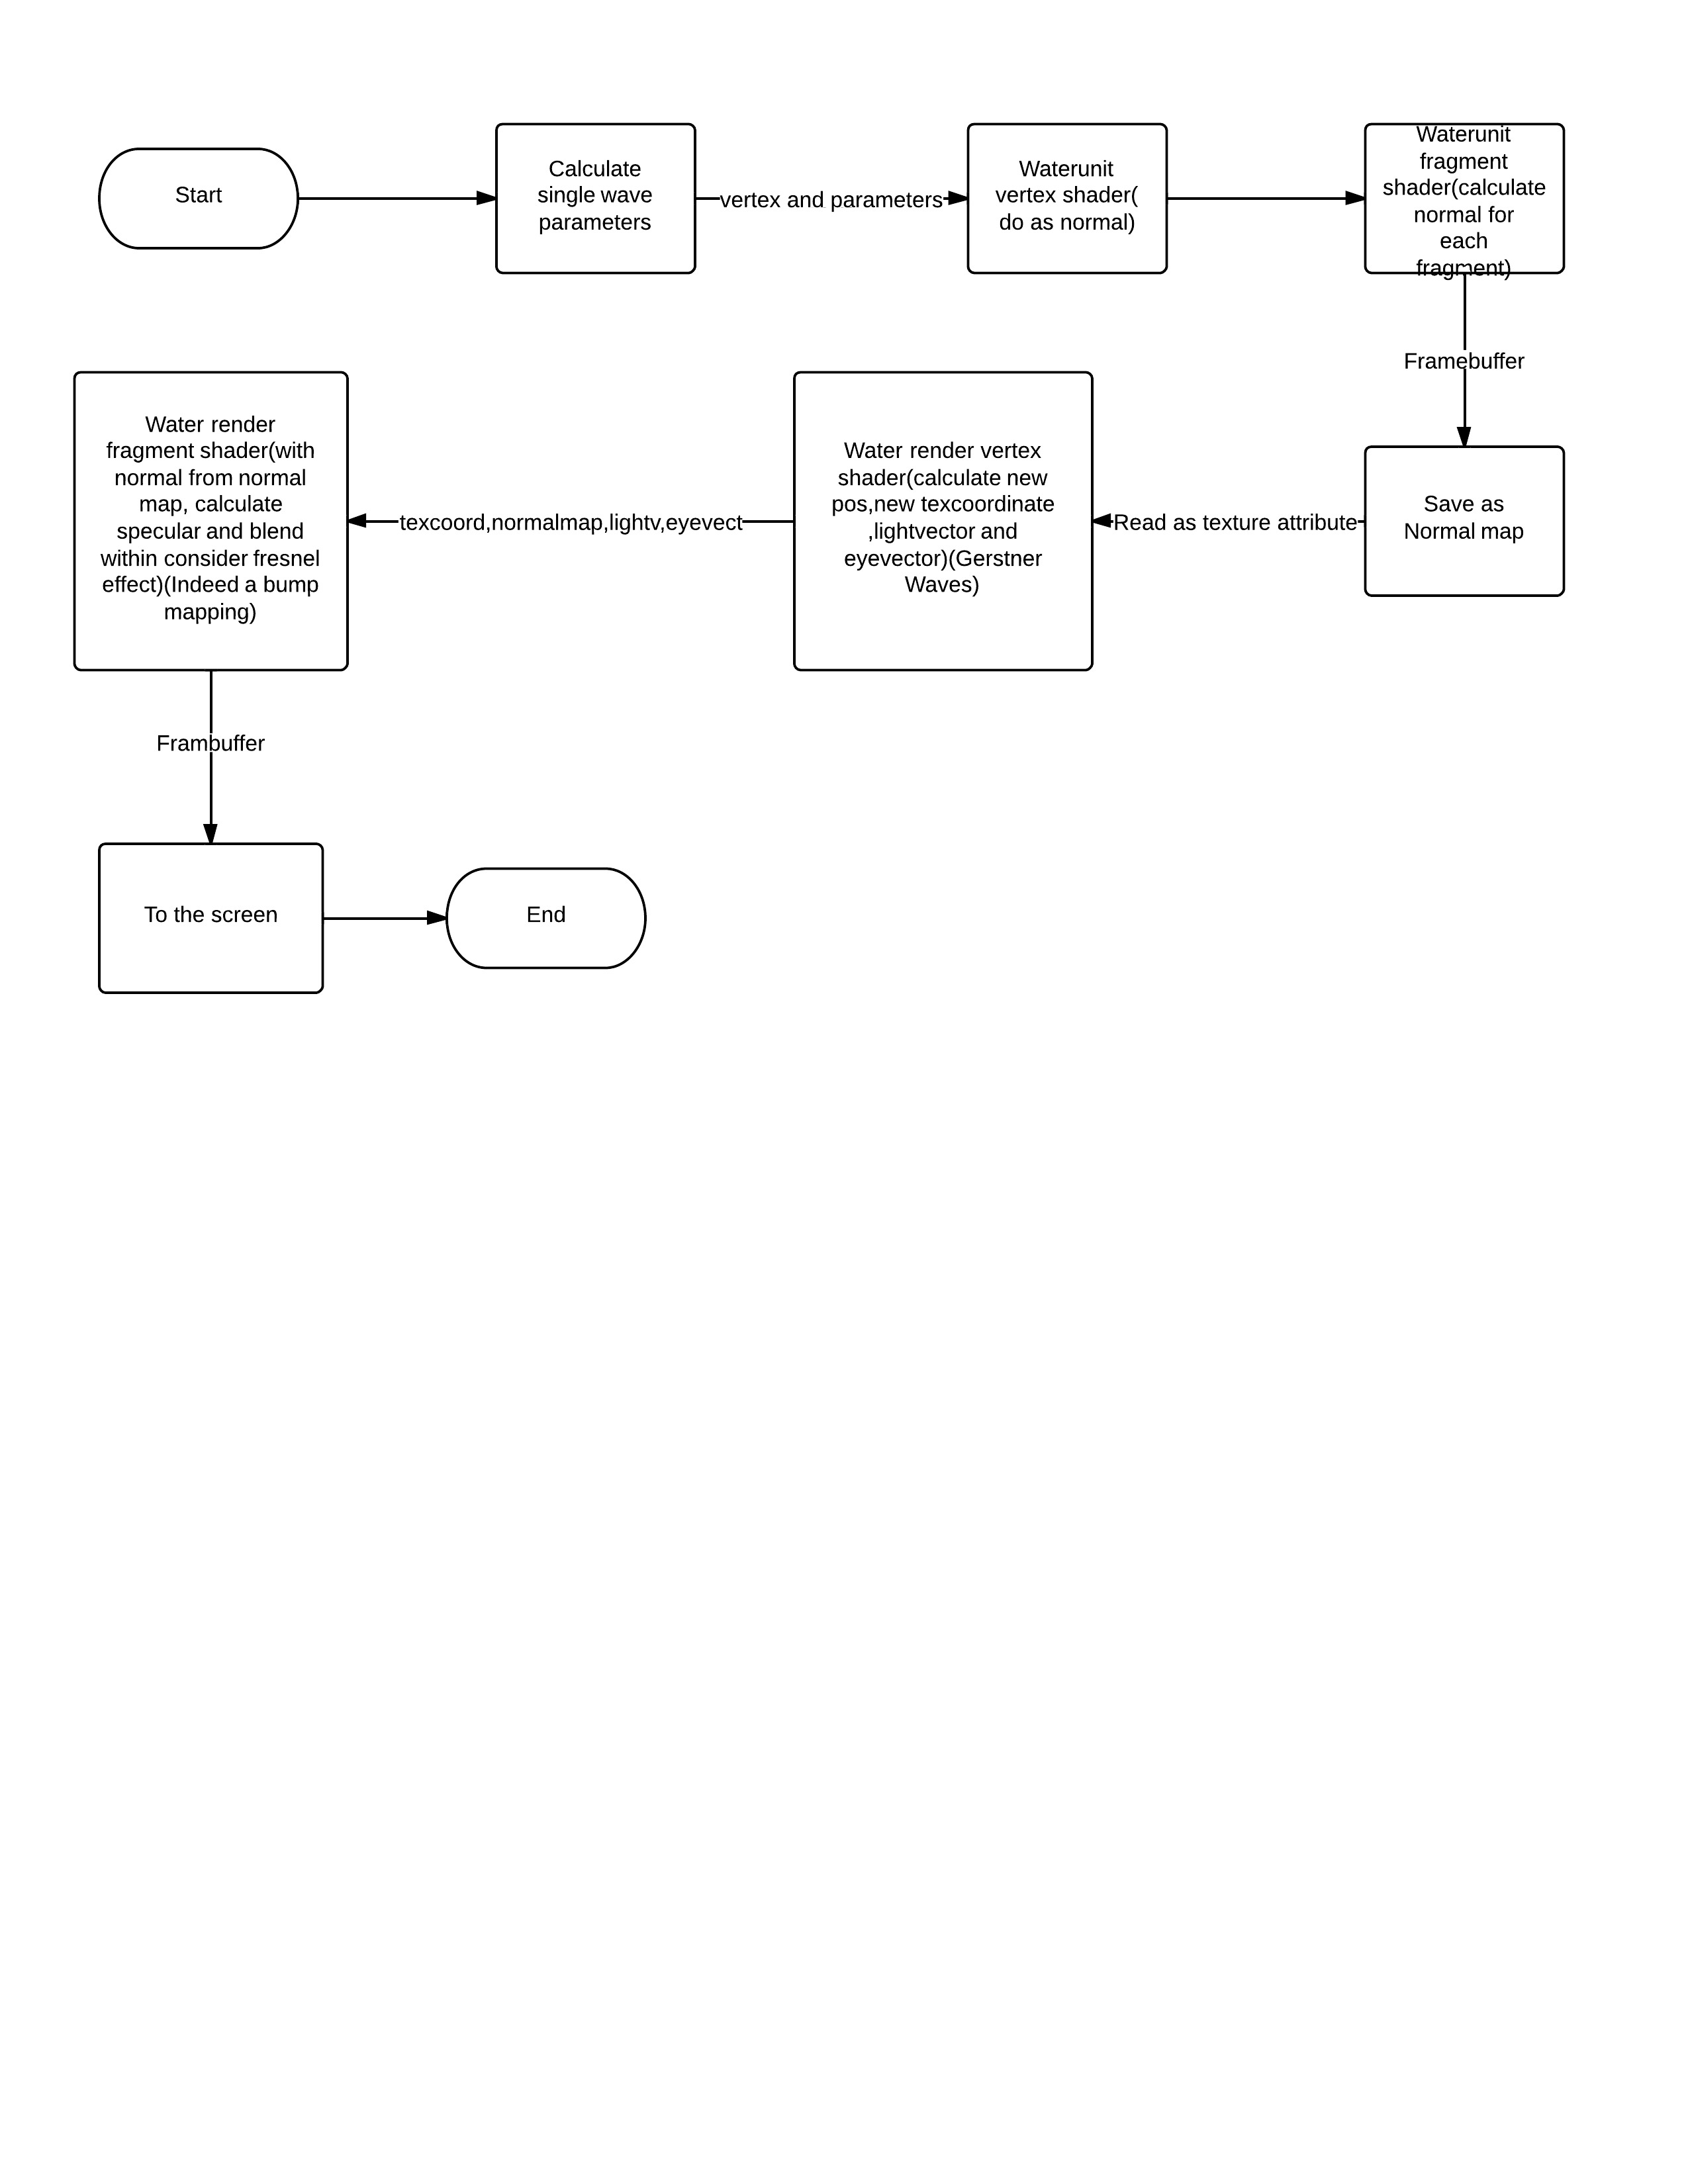
\includegraphics[width=1.0\textwidth]{flow.jpeg}
    \caption{A flow chart}
\end{figure}
\begin{figure}[p]
    \centering
    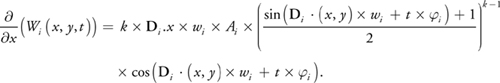
\includegraphics[width=1.0\textwidth]{fig2.jpg}
    \caption{normal equation}
\end{figure}
\begin{figure}[p]
    \centering
    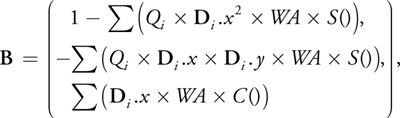
\includegraphics[width=1.0\textwidth]{B.jpg}
    \caption{bi-normal equation Gerstner Waves}
\end{figure}
\begin{figure}[p]
    \centering
    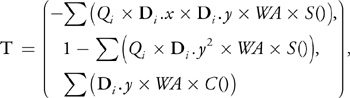
\includegraphics[width=1.0\textwidth]{T.jpg}
    \caption{tangent equation Gerstner Waves}
\end{figure}
\begin{figure}[p]
    \centering
    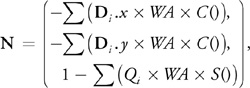
\includegraphics[width=1.0\textwidth]{N.jpg}
    \caption{normal equation Gerstner Waves}
\end{figure}

\section{some results}
\begin{figure}[p]
    \centering
    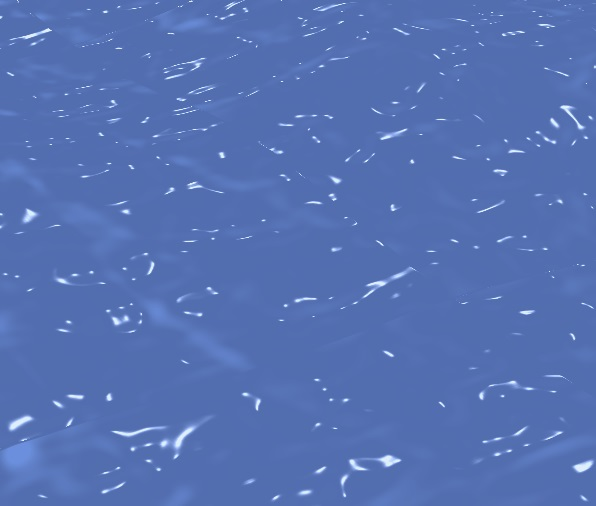
\includegraphics[width=1.0\textwidth]{unitwater.jpg}
    \caption{this is to show how a unit water looks like, not what waterunit.frag gives out(that is normal maps nor a frame buffer)}
\end{figure}
\begin{figure}[p]
    \centering
    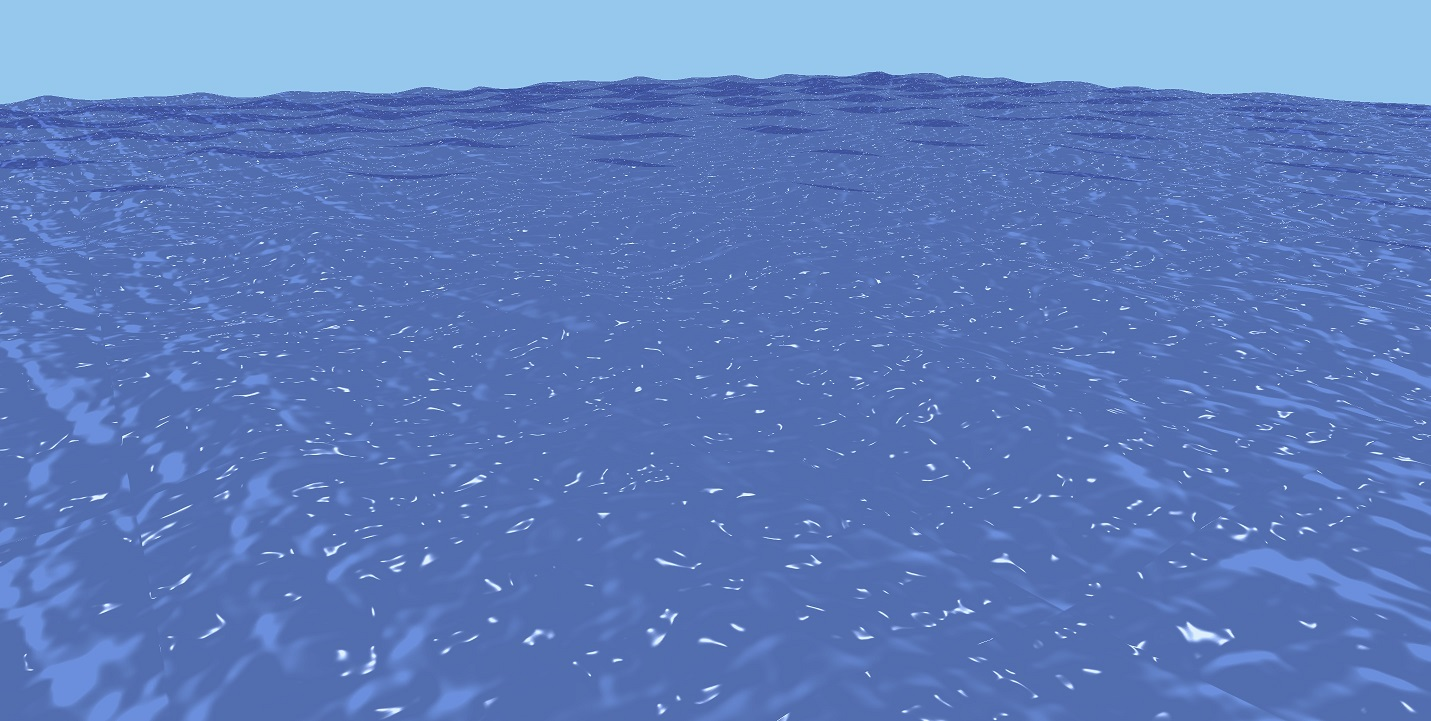
\includegraphics[width=1.0\textwidth]{wideview.jpg}
    \caption{from a far pos look at the water}
\end{figure}
\begin{figure}[p]
    \centering
    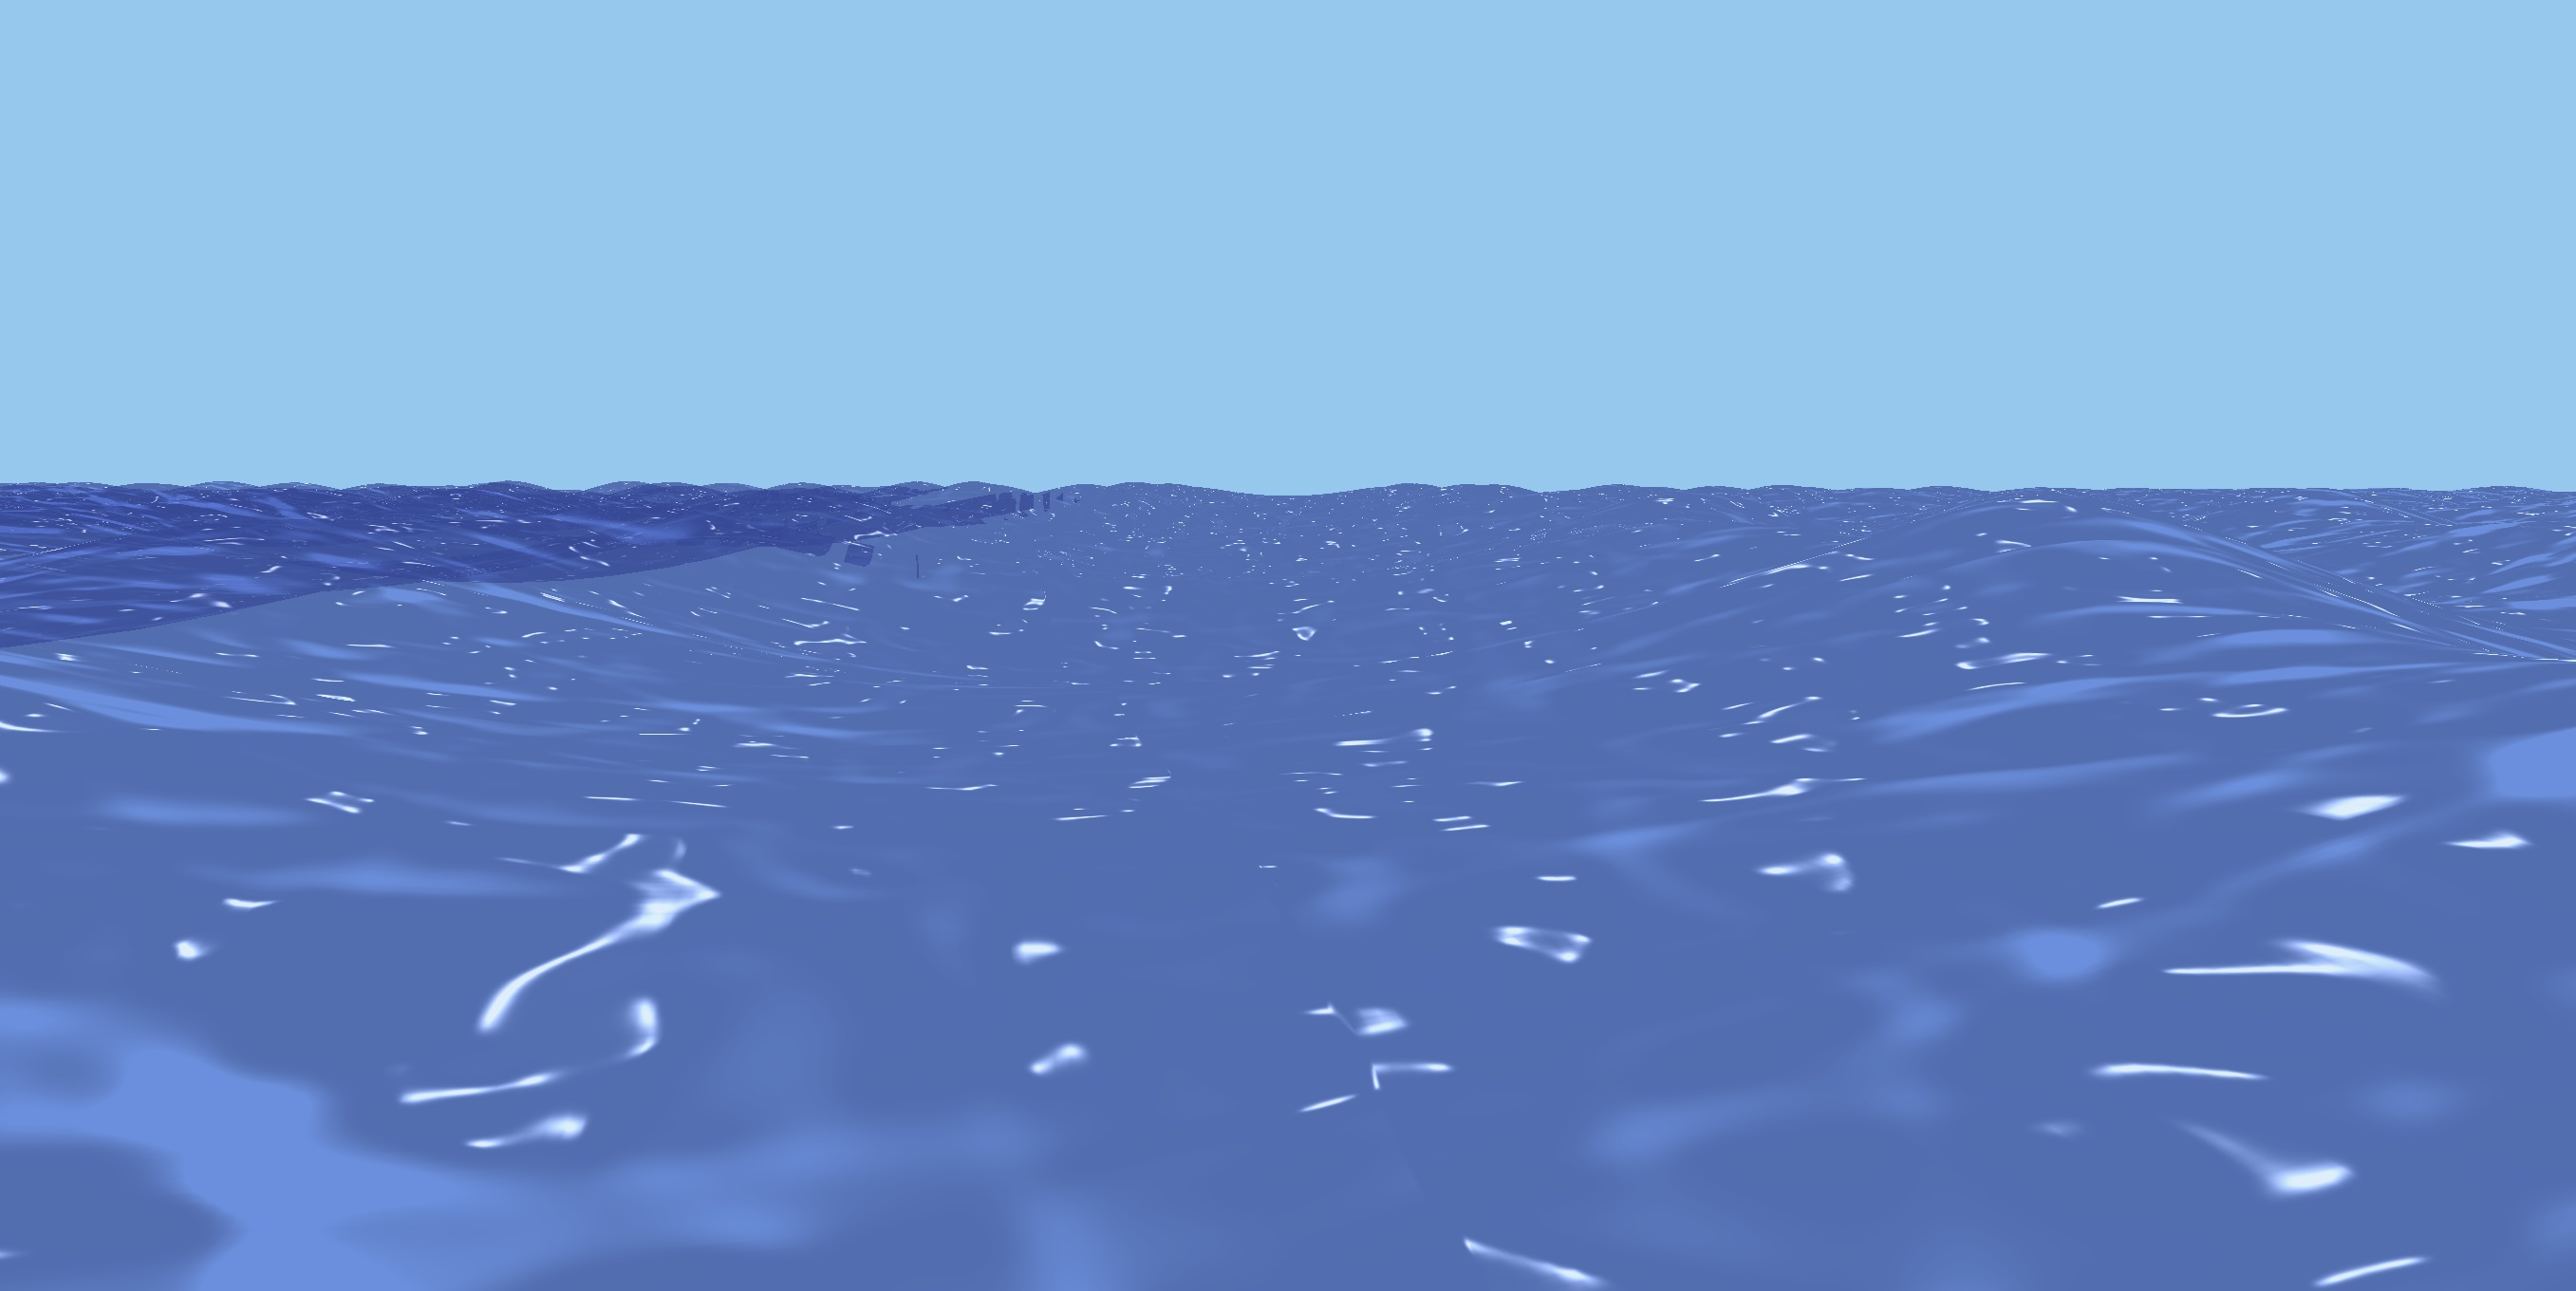
\includegraphics[width=1.0\textwidth]{closeview.jpg}
    \caption{from a close pos look at the water}
\end{figure}
\begin{figure}[p]
    \centering
    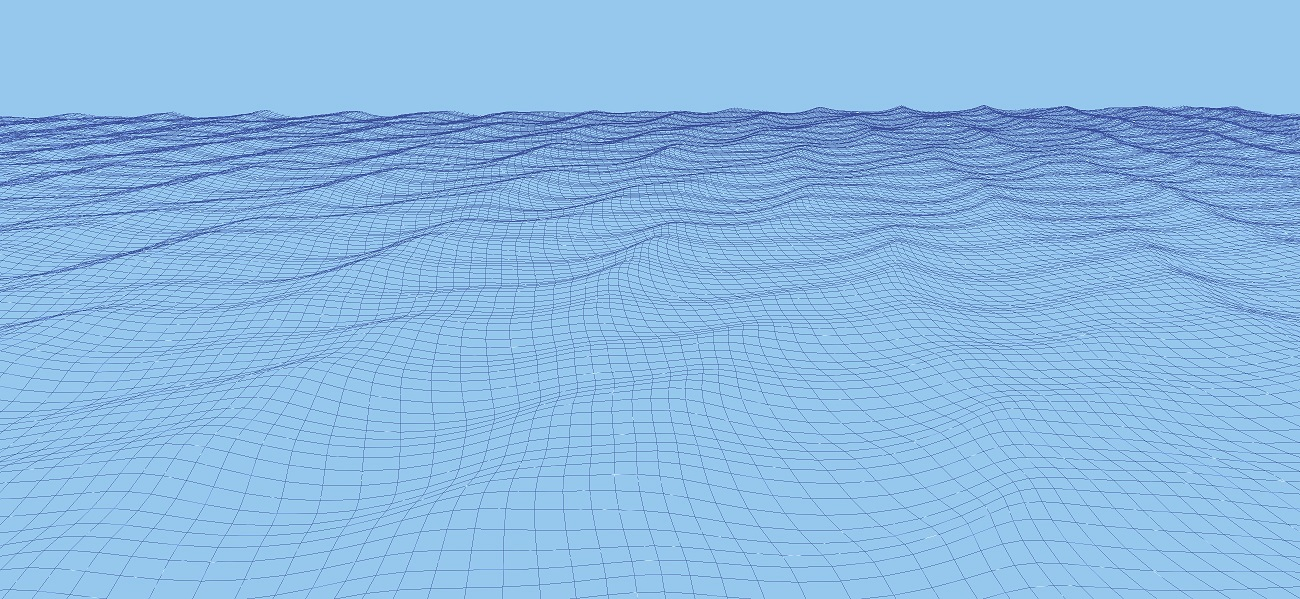
\includegraphics[width=1.0\textwidth]{geometry.jpg}
    \caption{show how the geometry of the water looks like}
\end{figure}



\end {document}
